\chapter{IRRADIANCE NETWORK FORECASTS}
\label{chap:network}

Reference other sections


Background from vincent, how it's done, limitations, possible
improvements

\section{Basic Summary}
\begin{figure}[h]
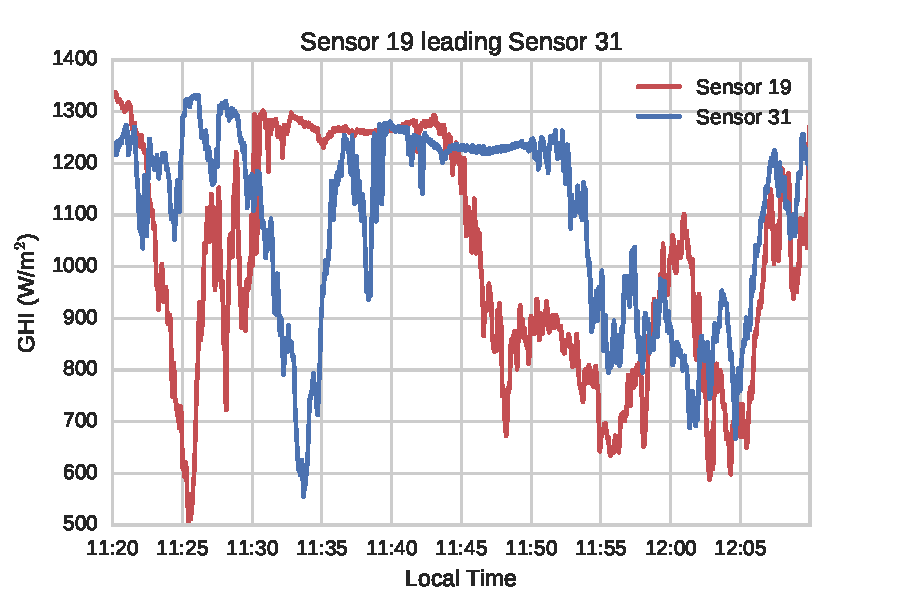
\includegraphics[width=\textwidth]{figs/leading_sens.pdf}
\caption[Example of data from one sensor predicting the output of
another]{An example of the output of sensor 19 (red) predicting what
  the output of the upstream sensor 31 (blue) in roughly 8
  minutes.}
\label{fig:leading_sens}
\end{figure}


new methods in this area

\section{Irradiance Forecast Error Metrics}
\label{sec:error_metrics}
regional comparisons

time errors

standard metrics
mae vs rmse vs mbe

other metrics

make PDFs?

\begin{figure}[h]
\centering
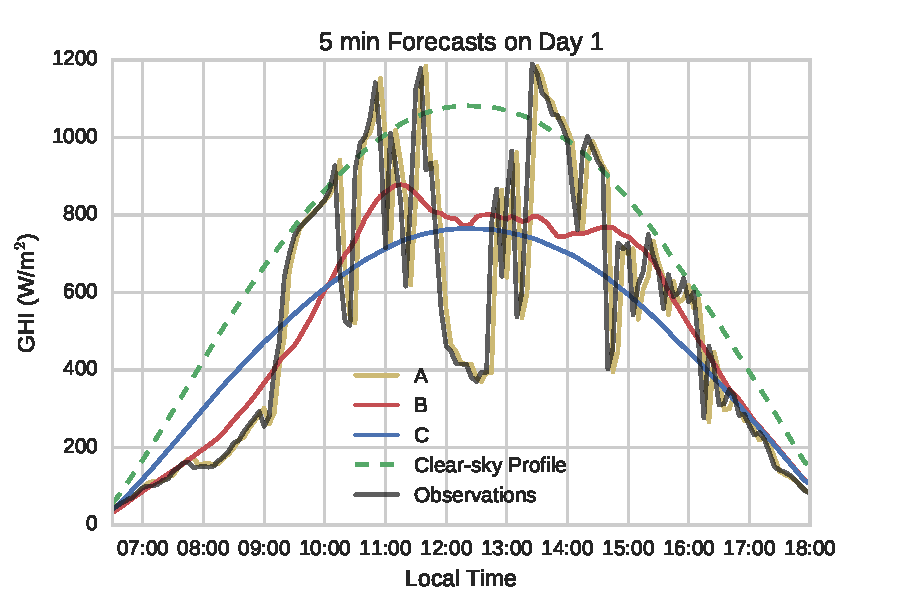
\includegraphics[width=0.8\textwidth]{figs/error_fx_Day_1.pdf}
\caption[Forecasts for a day with thick, broken clouds]{Five minute
  ahead forecasts for a day with thick broken clouds. Forecast A is a
  persistence forecast that captures the variability of the
  observations, but offset by 5 minutes. Forecast B is a somewhat
  smoothed forecast, and Forecast C is simply a fraction of the
  clear-sky profile.}
\label{fig:5minfx_day1}
\end{figure}


\begin{figure}[h]
\centering
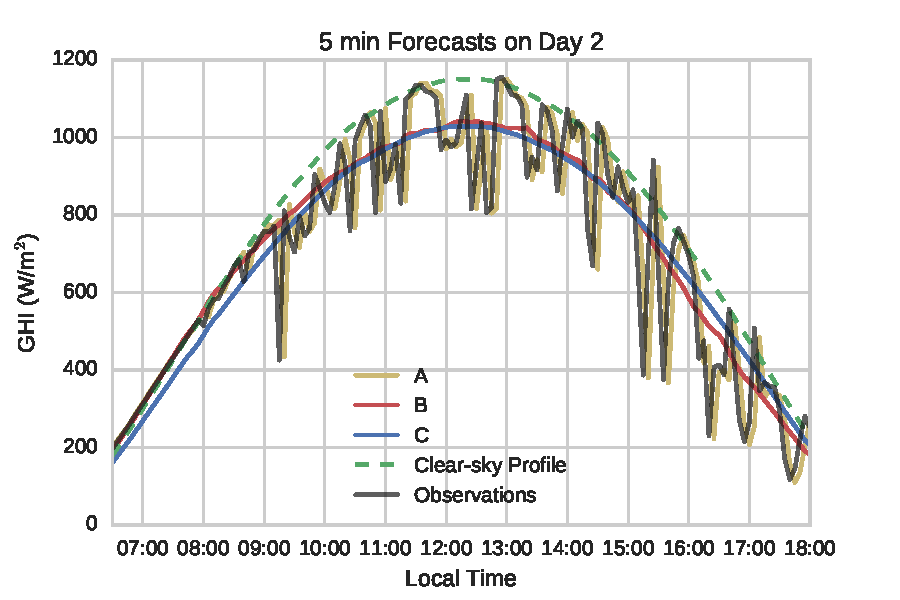
\includegraphics[width=0.8\textwidth]{figs/error_fx_Day_2.pdf}
\caption[Forecasts for a day with scattered clouds]{Five minute
  ahead forecasts for a day with scattered clouds. Forecast A is a
  persistence forecast that captures the variability of the
  observations, but offset by 5 minutes. Forecast B is a somewhat
  smoothed forecast, and Forecast C is simply a fraction of the
  clear-sky profile.}
\label{fig:5minfx_day2}
\end{figure}

\begin{table}[h]
\centering
\caption[Error metrics for example forecasts]{Error metrics (in units
of clear-sky index) for the forecasts on Day 1 shown in
\cref{fig:5minfx_day1} and Day 2 shown in
\cref{fig:5minfx_day2}. Refer to the text of \cref{sec:error_metrics}
for a description of each metric.}
\label{table:fx_errs}
\vspace{.3em}
\captionsetup{position=top}
\subfloat[Day 1\label{table:fx_errs_day1}]{\input{figs/Day_1_err_table}}
\hspace{3em}
\subfloat[Day 2\label{table:fx_errs_day2}]{\input{figs/Day_2_err_table}}
\end{table}


\subsection{Taylor Diagrams}

\begin{figure}[h]
\centering
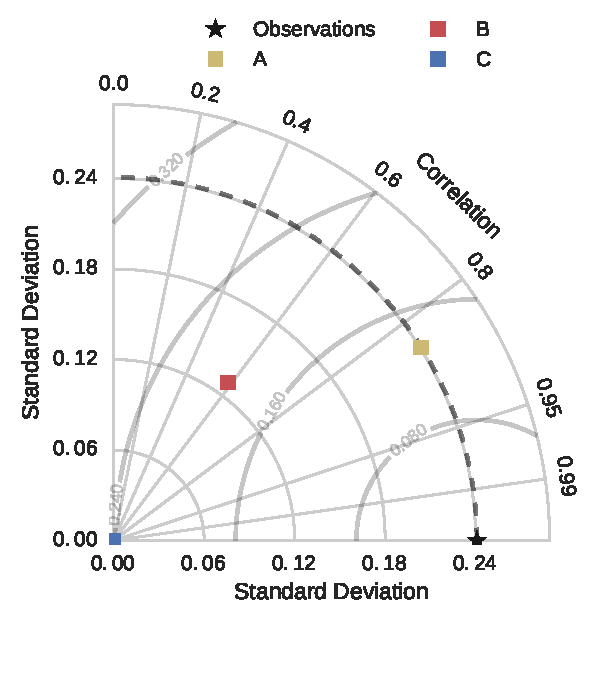
\includegraphics[width=0.8\textwidth]{figs/taylor_Day_1.pdf}
\vspace{-3em}
\caption[Taylor diagram for day 1 example forecasts]{A Taylor diagram
  for the forecasts on Day 1 shown in \cref{fig:5minfx_day1}. The
  light gray contours are lines of constant CRMSE. Forecast A has the
  lowest CRMSE in addition to having the same variability, as measured
  by the standard deviation, as the observations.}
\label{fig:taylor_day1}
\end{figure}

\begin{figure}[h]
\centering
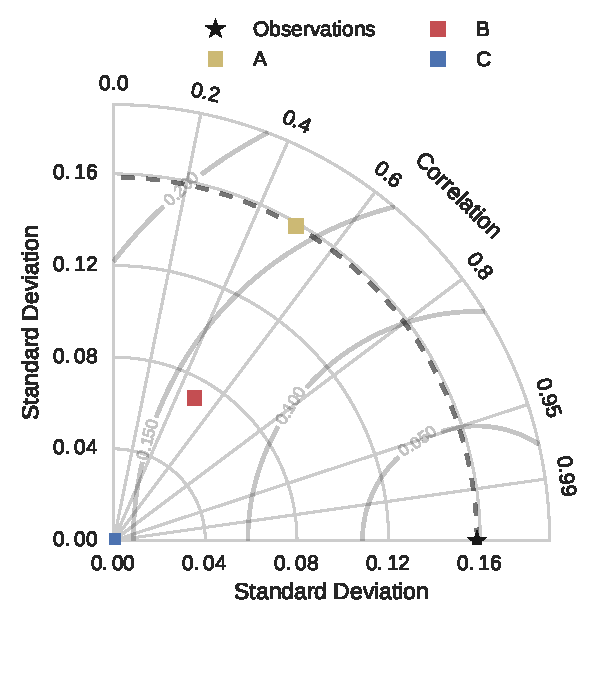
\includegraphics[width=0.8\textwidth]{figs/taylor_Day_2.pdf}
\vspace{-3em}
\caption[Taylor diagram for day 2 example forecasts]{A Taylor diagram
  for the forecasts on Day 2 shown in \cref{fig:5minfx_day2}. On this
  day, Forecast B has a smaller CRMSE and about the same correlation
  as Forecast A. However, Forecast A has similar variability to the
  observations as measured by the standard deviation. Depending on
  what the intended use of the forecast is, Forecast A may be the
  ``better'' forecast.}
\label{fig:taylor_day2}
\end{figure}


\section{Future Work}
velocity vectors

ensemble kalman filter

domain specific prediction

%%% Local Variables:
%%% mode: latex
%%% TeX-master: "dissertation"
%%% End:
